%$Id: chi06.tex,v 1.4 2006/02/13 23:19:21 rlw Exp rlw $
\documentclass[dvips]{beamer}
\usetheme[hideothersubsections]{Boston}
\usepackage{amsmath,amssymb,bm,array,graphicx,epic,hyperref,url,psfrag}
\usepackage{multirow, dcolumn}
%\usepackage{movie15}
%\bibliographystyle{jasa}
\graphicspath{{./}{eps/}}
\setbeamercovered{transparent}
\title{Bayesian Nonparametric Models}
\subtitle{\Large  using Levy Random Fields and Overcomplete Dictionaries}
\author[M. Clyde]{Merlise Clyde}
\institute{Department of Statistical Science \\ Duke
University }
\date{WISE June 5, 2011}
\newcommand{\bs}[2]{\begin{frame} \frametitle{#1} 
{#2}
\end{frame} }
\usepackage{amsmath,amssymb,array,eucal}
\usepackage{xcolor}
\definecolor{beamer@blendedblue}{RGB}{86,155,189}
\definecolor{myblue}{RGB}{12,76,138}
\setbeamercolor{structure}{fg=myblue}
\definecolor{Ftitle}{RGB}{12,76,138}
\definecolor{Descitem}{RGB}{238,238,244}
\definecolor{StdTitle}{RGB}{12,76,138}
\definecolor{StdBody}{RGB}{213,24,0}
\definecolor{StdBody}{RGB}{213,24,0}

\definecolor{AlTitle}{RGB}{255, 190, 190}
\definecolor{AlBody}{RGB}{213,24,0}

\definecolor{ExTitle}{RGB}{201, 217, 217}
\definecolor{ExBody}{RGB}{213,24,0}

\setbeamercolor{frametitle}{fg = Ftitle}
\setbeamercolor{title}{fg = Ftitle}
\setbeamercolor{item}{fg = Ftitle}
\setbeamercolor{subitem}{fg = Ftitle}
\setbeamercolor{subsubitem}{fg = Ftitle}
\setbeamercolor{description item}{fg = myblue}
\setbeamercolor{titlelike}{fg=myblue}
\newcommand{\e}{\mathbf{e}}
\renewcommand{\P}{\textsf{P}}
\newcommand{\R}{\textsf{R}}
\newcommand{\mat}[1] {\mathbf{#1}}
%\newcommand{\ind}{\mathrel{\mathop{\sim}\limits^{\mathit{ind}}}}
%\newcommand{\iid}{\mathrel{\mathop{\sim}\limits^{\mathit{iid}}}}
\newcommand{\E}{\textsf{E}}
\newcommand{\SE}{\textsf{SE}}
\newcommand{\SSE}{\textsf{SSE}}
\renewcommand{\SS}{\textsf{SS}}
\newcommand{\MSE}{\textsf{MSE}}
\newcommand{\SSR}{\textsf{SSR}}
\newcommand{\Be}{\textsf{Beta}}
\newcommand{\St}{\textsf{St}}
%\newcommand{\C}{\textsf{C}}
\newcommand{\GDP}{\textsf{GDP}}
\newcommand{\NcSt}{\textsf{NcSt}}
\newcommand{\Bin}{\textsf{Bin}}
\newcommand{\NB}{\textsf{NegBin}}
\renewcommand{\NG}{\textsf{NG}}
\newcommand{\N}{\textsf{N}}
\newcommand{\Ber}{\textsf{Ber}}
\newcommand{\Poi}{\text{Poi}}
\newcommand{\Gam}{\textsf{Gamma}}
\newcommand{\Gm}{\textsf{G}}
\newcommand{\Un}{\textsf{Unif}}
\newcommand{\Ex}{\textsf{Exp}}
\newcommand{\DE}{\textsf{DE}}
\newcommand{\tr}{\textsf{tr}}
\newcommand{\cF}{{\cal{F}}}
\newcommand{\cL}{{\cal{L}}}
\newcommand{\cI}{{\cal{I}}}
\newcommand{\cB}{{\cal{B}}}
\newcommand{\cP}{{\cal{P}}}
\newcommand{\bbR}{\mathbb{R}}
\newcommand{\bbN}{\mathbb{N}}
\newcommand{\pperp}{\mathrel{{\rlap{$\,\perp$}\perp\,\,}}}
\newcommand{\OFP}{(\Omega,\cF, \P)}
\newcommand{\eps}{\boldsymbol{\epsilon}}
\newcommand{\1}{\mathbf{1}_n}
\newcommand{\gap}{\vspace{8mm}}
\newcommand{\ind}{\mathrel{\mathop{\sim}\limits^{\rm ind}}}
\newcommand{\simiid}{\ensuremath{\mathrel{\mathop{\sim}\limits^{\rm
iid}}}}
\newcommand{\eqindis}{\ensuremath{\mathrel{\mathop{=}\limits^{\rm D}}}}
\newcommand{\iid}{\textit{i.i.d.}}
\newcommand{\SSZ}{S_{zz}}
\newcommand{\SZW}{S_{zw}}
\newcommand{\Bias}{\textsf{Bias}}
\newcommand{\Var}{\textsf{Var}}
\newcommand{\corr}{\textsf{corr}}
\newcommand{\diag}{\textsf{diag}}
\newcommand{\var}{\textsf{var}}
\newcommand{\Cov}{\textsf{Cov}}
\newcommand{\Sam}{{\cal S}}
\def\H{\mathbf{H}}
\newcommand{\I}{\mathbf{I}}
\newcommand{\Y}{\mathbf{Y}}
\newcommand{\tY}{\tilde{\mathbf{Y}}}
\newcommand{\Yhat}{\hat{\mathbf{Y}}}
\newcommand{\Yobs}{\mathbf{Y}_{{\cal S}}}
\newcommand{\barYobs}{\bar{Y}_{{\cal S}}}
\newcommand{\barYmiss}{\bar{Y}_{{\cal S}^c}}
\def\bv{\mathbf{b}}
\def\X{\mathbf{X}}
\def\tX{\tilde{\mathbf{X}}}
\def\x{\mathbf{x}}
\def\xbar{\bar{\x}}
\def\Xg{\mathbf{X}_{\boldsymbol{\gamma}}}
\def\Ybar{\bar{Y}}
\def\ybar{\bar{y}}
\def\y{\mathbf{y}}
\def\Yf{\mathbf{Y_f}}
\def\W{\mathbf{W}}
\def\w{\mathbf{w}}
\def\U{\mathbf{U}}
\def\V{\mathbf{V}}
\def\Q{\mathbf{Q}}
\def\Z{\mathbf{Z}}
\def\z{\mathbf{z}}
\def\v{\mathbf{v}}
\def\u{\mathbf{u}}

\def\zero{\mathbf{0}}
\def\one{\mathbf{1}}
\newcommand{\taub}{\boldsymbol{\tau}}
\newcommand{\betav}{\boldsymbol{\beta}}
\newcommand{\alphav}{\boldsymbol{\alpha}}
\newcommand{\A}{\mathbf{A}}
\def\a{\mathbf{a}}
\newcommand{\B}{\mathbf{B}}
\def\b{\boldsymbol{\beta}}
\def\bhat{\hat{\boldsymbol{\beta}}}
\def\tb{\tilde{\boldsymbol{\beta}}}
\def\bg{\boldsymbol{\beta_\gamma}}
\def\bgnot{\boldsymbol{\beta_{(-\gamma)}}}
\def\mub{\boldsymbol{\mu}}
\def\tmub{\tilde{\boldsymbol{\mu}}}
\def\muhat{\hat{\boldsymbol{\mu}}}
\def\t{\boldsymbol{\theta}}
\def\tk{\boldsymbol{\theta}_k}
\def\tj{\boldsymbol{\theta}_j}
\def\Mk{\boldsymbol{{\cal M}}_k}
\def\M{{{\cal M}}}
\def\Mj{{{\cal M}}_j}
\def\Mi{{{\cal M}}_i}
\def\Mg{{\cal M}_\gamma}
\def\Mnull{{\cal M}_{N}}
\def\gMPM{\boldsymbol{\gamma}_{\text{MPM}}}
\def\gHPM{\boldsymbol{\gamma}_{\text{HPM}}}
\def\Mfull{\boldsymbol{{\cal M}}_{F}}
\def\tg{\boldsymbol{\theta}_{\boldsymbol{\gamma}}}
\def\g{\boldsymbol{\gamma}}
\def\eg{\boldsymbol{\eta}_{\boldsymbol{\gamma}}}
\def\G{\mathbf{G}}
\def\cM{\cal M}
\def\D{\Delta}
\def \shat{{\hat{\sigma}}^2}
\def\uv{\mathbf{u}}
\def\l {\lambda}
\def\d{\delta}
\def\Sigmab{\boldsymbol{\Sigma}}
\def\Lambdab{\boldsymbol{\Lambda}}
\def\lambdab{\boldsymbol{\lambda}}
\def\Mg{{\cal M}_\gamma}
\def\S{{\cal{S}}}
\def\qg{p_{\boldsymbol{\gamma}}}
\def\pg{p_{\boldsymbol{\gamma}}}
\def\t{\boldsymbol{\theta}}
\def\T{\boldsymbol{\Theta}}

\input{colornames}
\newcommand{\blue}{\textcolor{Blue}}
\newcommand{\green}{\textcolor{PineGreen}}
\newcommand{\purple}{\textcolor{Purple}}
\newcommand{\red}{\textcolor{RedOrange}}
\definecolor{aper}{rgb}{0.7412,0,1}
\definecolor{daily}{rgb}{0.1412,0,1}
\newcommand{\ap}{\textcolor{aper}}
\newcommand{\dy}{\textcolor{daily}}
\logo{
\includegraphics[width=.6in,height=.6in]{duke}}


\begin{document}
\begin{frame}
  \titlepage
\end{frame}
%\section[Outline]{}

%\bs{Outline}{
%\tableofcontents 
%}

\section{Nonparametric Regression}
\bs{Problem Setting}{
Consider the nonparametric regression problem where we observe
noisy measurements  $\{Y_i\} \quad i \in  I $ of an
unknown function $f(\bfx): \cfX \to \bbR$
$$ \E[Y \mid \bfx] = f(\bfx), \quad \bfx \in \cfX$$


Need flexible prior distributions on functions 


Usual Suspects: 
\begin{itemize}
\item  Gaussian Process Priors
\item  Dirichlet Process priors
\item  Expansions of $f$  
\end{itemize}


\vfill

Focus on L\'evy Processes!  (related to GP \& DP)
}

\bs{Goals} {
  \begin{itemize}
  \item ``Machine Learning'' Classification/Prediction problems
  \item Learning ``features'' of $f$ 
    \begin{itemize}
    \item  which variables in $\bfx$ are
      important for classification
    \item location of peaks/proteins in spectra
    \item sources/spread of pollutants in space/time models
    \end{itemize}
  \end{itemize}

\vspace{-.25in}
\centerline{  \includegraphics[height=2in]{mean-spectrum.ps}}

\vspace{-.25in}
Deconvolution problem 
}

\bs{Multiple Spectra} {
\begin{center}
\begin{tabular}{cc}
\includegraphics[height=1in,angle=-90]{RawSpecCont_n4_allFrcAvg_22.ps}&
\includegraphics[height=1in,angle=-90]{RawSpecDis_n15_allFrcAvg_22.ps}\vspace{-.2in}\\
\includegraphics[height=1in,angle=-90]{RawSpecCont_n2_allFrcAvg_22.ps}&
\includegraphics[height=1in,angle=-90]{RawSpecDis_n14_allFrcAvg_22.ps}\vspace{-.2in}\\
\includegraphics[height=1in,angle=-90]{RawSpecCont_n1_allFrcAvg_22.ps}&
\includegraphics[height=1in,angle=-90]{RawSpecDis_n11_allFrcAvg_22.ps}
%\includegraphics[angle=-90]{/proj/levy/proteomics/multiSpec_paper/paper_figures/RawSpecCont_Frc5_subset.ps}&
%\includegraphics[angle=-90]{/proj/levy/proteomics/multiSpec_paper/paper_figures/RawSpecDis_Frc5_subset.ps}\\
\end{tabular}
\end{center}

Learning ``features'' that are common versus those that separate groups of  functions (spectra)

}

\bs{Stochastic Expansions} {

Expand $f(\bfx_i) = \sum_{j=0}^{J}  \psi_j(\bfx_i)\beta_j$ in
terms of an Overcomplete Dictionary where
 
  \begin{itemize}
   \item  $\{\psi_j\}$: dictionary elements
   \item  $\{\beta_j\}$:  unknown coefficients
   \item  $J$: number of elements in expansion (finite and infinite)
  \end{itemize}

Advantages: may lead to more flexibility in choosing ``building''
blocks to match features than GP or DP models.

\vspace{20pt}
How should we choose prior distributions so that the resulting $f$ is
well defined with desired smoothness properties?

}



\bs{Finite Expansions} {

Consider finite expansions for some collection  $J$ of dictionary elements
$\psi_j$

\begin{eqnarray*}
f(\bfx) &  = &  \sum_{j\le J}\psi_j(\bfx) \beta_j  \quad \quad  \{ \psi_j \in \cfF \}
\end{eqnarray*}

Independent scale mixtures of normals (Generalized Ridge Priors) 
\begin{eqnarray*}
  \beta_j \mid \varphi_j & \ind & \No(0,  \varphi_j^{-1}) \\
  \varphi_j    & \iid & \Ga(a, b) \\
\end{eqnarray*}

Tipping considers modal estimates in the case $a = b = 0$  

\blue{Improper prior and posterior!}
}
\bs{Model Selection Priors} {
For selection of dictionary elements from a Bayesian perspective, add
a point mass at zero in the distribution for $\beta_j$
\begin{eqnarray*}
  \beta_j \mid \varphi_j & \ind & \No(0, \gamma_j \varphi_j^{-1}) \\
  \varphi_j    & \iid & \Ga(a, b) \\
  \gamma_j & \iid & \Ber(\pi)
\end{eqnarray*}
\begin{itemize}
\item Choice of  global scale as $J$ increases?
\item Choice of $\pi$ as $J$ increases? 
\item Number of non-zero
  coefficients is Binomial with mean $J \pi$.
Limit as $J \to \infty$ such that $J \pi \to \nu_+$ is
  Poisson with mean $\nu_+$
\end{itemize}

Consider model to unify finite and infinite dimensional models!
}

\bs{L\'evy Priors} {
Hierarchical Student-$t$ prior
\begin{eqnarray*}
  \beta_j \mid \varphi_j & \ind & \No(0,  \varphi_j^{-1}) \\
  \varphi_j    & \ind & \Ga\left(\frac{\alpha}{2}, \frac{\alpha \epsilon^2}{2}\right) \\
   J & \sim & \Po(\nu^+_\epsilon)
\end{eqnarray*}
where $\nu^+_\epsilon = \nu_\epsilon(\bbR) = \frac{\alpha ^{1
    - \alpha/2} \Gamma(\alpha)\Gamma(\alpha/2)}{\epsilon^\alpha
  \pi^{1/2} \Gamma(\frac{\alpha +1}{2})} \sin(\frac{\pi \alpha} {2})$

\vspace{.5in}
Limit as $\epsilon \to 0$ leads to \Levy\ $alpha$-Stable process!
}

\bs{L\'evy Adaptive Regression Kernels} {
Stochastic Integral Representation 
\begin{align*}
f(x)   & =   \sum_{j\le J}\psi(\bfx; \bfomega_j) \beta_j \equiv \int_{\bfOmega}  
\psi(x;\bfomega) \Lmea(d\bfomega) \\
\psi(\bfx,\bfomega_j) & \equiv g( \bfLambda_j (\bfx - \mean_j))
\quad \text{"generator"}
\end{align*} 


$\Lmea$ is a Signed Measure:
$$\Lmea(d\bfomega)  = \sum_{j\le J} \beta_j \delta_{\bfomega_j}(d\bfomega) $$

  \begin{itemize}
 
  \item  support points of $\Lmea$: $\{\bfomega_j\} = \{\mean_j,\scale_j\}$ 
    \begin{itemize}
    \item``location'' parameters:  $\mean_j\in\cfX$  
    \item ``scaling'' parameters:  $\scale_j\in\bbR^+$  
    \end{itemize} 
  \item jump sizes of measure:  $\beta_j$   
  \item number of support points  $J$ 
  \end{itemize}
} 

\bs{Generators} {
Dictionary elements generated by $\psi(\bfx,\bfomega_j)  \equiv g(
\bfLambda_j (\bfx - \mean_j))$ translation and scaling as in wavelets
  \begin{itemize}
  \item kernels  (as in kernel regression or SVM)
  \item densities of location-scale families  Gaussian or Cauchy
    kernel (for mass spect)
  \item exponential densities  (pollutant concentrations) 
  \item wavelet families
  \end{itemize}
No need for symmetric kernels as in SVM

Generates \blue{continuous} dictionaries
}
\subsection{L\'evy Random Field Priors }

\bs{ L\'evy  Random Fields} {
  \begin{itemize}
  \item 
$\Lmea(d\bfomega)$  is a \blue{random (signed) measure} on $\bfOmega$ 

\item Convenient to think of a random measure as stochastic process where
$\Lmea$ assigns random variables  to sets $A \in \bfOmega$

\item Take
$$\Lmea \sim \Lv(\nu) \text{ with L\'evy measure } \nu(d \beta, d
  \bfomega)$$
where $\nu$ satisfies integrability condition:
\end{itemize}
\begin{equation}
  \label{eq:l2-bound}
\int_{\bbR \times \Omega} \min(1, \beta^2) \, \nu(d\beta, d
  \bfomega) < \infty
\end{equation}


\blue{Poisson Representation} of L\'evy Random Fields is the key to
Bayesian Inference!
}

\bs{Poisson Representation}{ 
Goal: $f(x) = \sum_{j < J}  \psi(\bfx, \bfomega_j) \beta_j = \sum_{j <
  J} g(\Scale_j(\bfx - \mean_j))$ 

\blue{Sufficient condition} for bounded $\k$:
\begin{equation}
  \label{eq:l1-bound}
\int_{\bbR \times \Omega} \min(1, |\beta|) \nu(d\beta, d
  \bfomega) < \infty
\end{equation}

\begin{itemize}
\item[$\Rightarrow$] $J \sim \Po(\nu_+)$,\qquad $\nu_+\equiv
  \nu(\bbR\times\bfOmega)$
\item[$\Rightarrow$] $\beta_j,\bfomega_j \mid J \iid \pi(d\beta, d\bfomega)
  \propto \nu(d\beta,d\bfomega)$.
\end{itemize}

\begin{itemize}
  \item Finite number of ``big'' coefficients $|\beta_j|$  
  \item Possibly infinite number of $\beta \in [-\epsilon, \epsilon]$
  \item Coefficients $|\beta_j|$ are absolutely summable\footnote{need to add a term to
\blue{``compensate''} the infinite number of tiny jumps that are not
absolutely summable under the more general integrability condition \Eqn{eq:l2-bound}}

  \end{itemize}
}

\bs{Existence Theorem} {

\begin{theorem}
  Let $\nu$ be a L\'evy measure on $\bbR \times \Omega$ satisfying (\ref{eq:l2-bound}).  Then
  $f(\bfx)$ is well-defined if $ \psi(\omega) \equiv g(\Scale(\cdot -\loc))$ satisfies
\begin{subequations}\label{e:exist}
\begin{align}
   \iint_{[-1,1]^c\times\Omega} \big(1\wedge|\beta\psi(\omega)|\big)\,
                   \nu( \dbdo)&<\infty\label{e:exa}\\
   \iint_{[-1,1]\times\Omega} \big(|\beta\psi(\omega)|\wedge|
                                 \beta\psi(\omega)|^2\big)\,
                      \nu( \dbdo)&<\infty.\label{e:exb}
\end{align}
For $\nu$ satisfying \Eqn{eq:l1-bound} the condition simplifies
\begin{equation}
   \iint_{\bbR\times\Omega} \big(1\wedge|\beta\phi(\omega)|\big)\,
                   \nu( \dbdo)<\infty
\end{equation}

\end{subequations}

\end{theorem}
$g$ is  in a  ``Musielak-Orlicz space''

}

\bs{Function Spaces} {
The Besov space $\Besov$ consists of those $f\in
L_p(\bbR^d)$ whose Besov semi-norms are finite
\begin{equation} \label{e:besov-norm}
  \sspq{f} = \|f\|_p+\spq{f} < \infty
\end{equation}

For $p,q\ge0$ and $s> d(1/p - 1)_+$ and for any integer $m> s$ set
\begin{align}
\spq{f} &= \cet
      {\int_{|h|\le1} |h|^{-sq}\,\|\Delta^m_h f\|_p^q~  dh/|h|^d}^{1/q}\notag
\intertext{where $\Delta^m_h$ denotes
the $m$th forward finite difference,}
\Delta^0_h     f(x)&=f(x)\notag\\
\Delta^m_h f(x)&= \bet{\Delta^{m-1}_h f(x+h)-\Delta^{m-1}_hf(x)}\notag \\
 & = \sum_{k=0}^m \binom mk(-1)^{m-k} f(x + k h). \label{e:diff-sum}
\end{align}
}

\bs{LARK Models and Besov Spaces} {
Let $f(\bfx) = \int_\Omega \psi(\bfx, \omega) \Lmea(d \omega)$ where
$\psi(\bfx, \bfomega) = g(\Scale(\bfx - \loc))$ and $\Lmea \sim \Lv(\nu)$
\begin{theorem}
  Fix $\GB \in \Besov(\bbR^d)$ for some $p, q \ge 1$ and $s > 0$ and a \Levy\
  measure $\nu$ on $\bbR\times\Omega$ with $\Omega=(\LamS \times \bbR^d)$ of
  translation-invariant product form $\nu(\dbdo) = \nubw(d\beta\,
  d\Scale) d\loc$  for a $\sigma$-finite measure
  $\nubw (d\beta\, d\Scale)$ on $\bbR \times \LamS$ that satisfies the
  integrability condition \Eqn{eq:l1-bound} and the Existence Theorem.  Then 
  $f \in \Besov$ almost surely if $\nubw$ satisfies:
\begin{subequations}
\begin{align}
%  \iint_\RS \cet{1\wedge|\beta|} |\Scale|^{- 1}
%                \nubw(d\beta\, d\Scale)  < &\infty  \label{e:MO}\\
L_p: \quad  \iint_\RS \cet{1\wedge|\beta| |\Scale|^{- 1/p}}
                \nubw(d\beta\, d\Scale)  < &\infty  \label{e:Lp}\\
\Besov: \quad  \iint_\RS \cet{1\wedge|\beta| |\Scale|^{s - 1/p}}
                 \nubw(d\beta\, d\Scale)  < &\infty.  \label{e:Bspq}
\end{align}
\end{subequations}
\end{theorem}
}

\bs{L\'evy Measures} {

$\alpha$-Stable measure: $\nu(d\beta, d\bfomega) =  c_\alpha |\beta|^{-(\alpha
    +1)}\ \gamma(d\bfomega)$

For $\alpha$- Stable $\nu^+(\bbR, \bfOmega) = \infty$  

Fine in theory, but not in practice for MCMC!

\vspace{.25in}
Truncate measure to obtain a finite expansion:
\begin{itemize}
 \item The random number of support points $\bfomega$ with $\beta$ in $[-\epsilon, \epsilon]^c$ is finite
\item Fix $\epsilon$  (practical significance) 
\item Use approximate L\'evy  measure 
$$\nu_{\epsilon}(d\beta, d\bfomega) \equiv \nu(d\beta,
d\bfomega)\bfone(|\beta| > \epsilon) $$
\item[$\Rightarrow$] $J \sim \Po(\nu_{\epsilon}^+)$ where
  $\nu^+_{\epsilon} = \nu([-\epsilon, \epsilon]^c, \bfOmega)$
\item[$\Rightarrow$]  $\beta_j, \bfomega_j \iid \pi(d\beta, d\bfomega) \equiv
  \nu_\epsilon(d\beta , d \bfomega)/\nu^+_{\epsilon}$

\end{itemize}
}

\bs{Approximate L\'evy Prior} {
Continuous Approximation: 

$$\nu_\epsilon(d\beta, d \bfomega) = c_\alpha (\beta^2 + \alpha
\epsilon^2)^{-(\alpha + 1)/2} d\beta \ \gamma(d \bfomega) $$

Based on the following hierarchical prior
\begin{eqnarray*}
  \beta_j \mid \phi_j & \ind & \No(0,  \varphi_j^{-1}) \\
  \phi_j    & \ind & \Ga\left(\frac{\alpha}{2}, \frac{\alpha \epsilon^2}{2}\right) \\
   J & \sim & \Po(\nu^+_\epsilon)
\end{eqnarray*}
where $\nu^+_\epsilon = \nu_\epsilon(\bbR, \bfOmega) = \frac{\alpha ^{1
    - \alpha/2} \Gamma(\alpha)\Gamma(\alpha/2)}{\epsilon^\alpha
  \pi^{1/2} \Gamma(\frac{\alpha +1}{2})} \sin(\frac{\pi \alpha} {2}) \gamma(\bfOmega)$

\blue{Advantage}: Conjugate prior so $\beta$ can be integrated out for MCMC
}

\bs{Limiting Case} {
  \begin{eqnarray*}
    \beta_j   \mid  \varphi_j & \ind &\N(0, 1/\varphi_j) \\       
      \varphi_j & \iid & \Ga(\alpha/2, "0")
  \end{eqnarray*}

Notes:
  \begin{itemize}
\item Require $0 < \alpha < 2$ for characteristic function for $\Lmea$ and
  functionals to exist.  
\item  Cauchy corresponds to $\alpha = 1$
\item  Tipping's choice corresponds to $\alpha = 0$
\item Provides an extension of \blue{Generalized Ridge Priors}
      to infinite dimensional 
\item Infinite dimensional analog of Cauchy priors
 \end{itemize}
}


\section{Illustrations}
\subsection{Wavelet Examples}

\bs{Wavelet Test Functions (SNR = 7)} {
\begin{figure}[!h]
  \begin{center}
    \includegraphics[angle=270,origin=l,totalheight=6truecm,
     clip=1,width=10cm]{wavedata.ps}
  \end{center}
\end{figure}
}

\bs{Kernel Functions}{
\begin{figure}[!h]
  \begin{center}
    \includegraphics[angle=270,origin=l,totalheight=6truecm,
     clip=1,width=10cm]{kerplot.ps}
  \end{center}
\end{figure}
}

\bs{Comparisons of OCD Methods} {
  \begin{itemize}
  \item Translational Invariant Wavelets -- Laplace Priors
    (Johnstone \& Silverman     2005)  
  \item Continuous Wavelet Dictionary -- Compound Poisson with
    Gaussian Priors (Chu, Clyde, Liang 2007)
  \item LARK Symmetric Gamma
  \item LARK Cauchy
  \end{itemize}
Range of Over-complete Dictionaries and Priors
}
\bs{Comparison of Mean Square Error w/ OCDs} {
100 realizations of each function

\centerline{\includegraphics[width=2.5in,angle=270]{mse.eps} }
}
\subsection{MALDI-TOF}
\bs{MALDI-TOF Mass Spectroscopy} {
\begin{center}
\begin{tabular}[h]{{c}}
  \includegraphics[height=1.5in]{knownMean.2.75.both.ps} \\
  \includegraphics[height=1.5in]{known.res.vs.mz.both.ps} 
\end{tabular}

\end{center}

}
\subsection{Multivariate Features} 
\bs{Higher Dimensional $\cfX$} {

MCMC is too slow to allow
\begin{itemize}
\item location $\bfchi$ to be arbitrary; restrict to observed $\{\bfx_i\}$
\item scale parameter to vary with location; use common $\Lambda$
\item arbitrary $\Lambda$; restrict to diagonal $\Lambda$
\end{itemize}
\begin{eqnarray*}
k(\bfx, \bfomega_j) & = & \prod_d \exp\{ -\lambda_d (x_d - x_{jd})^2
\} \\  
f(\bfx) & =  & \sum_j k(\bfx, \bfomega_j) \beta_j
\end{eqnarray*}


\begin{itemize}
\item Product structure allows interactions between variables
\item Many input variables may be irrelevant
\item Feature selection; if $\lambda_d = 0$ variable $x_d$ is removed
\end{itemize}

}
\subsection{Regression Examples}
\bs{Regression Out of Sample Prediction} {
Average Relative MSE to best procedure
\small{
  \begin{tabular}[ht]{|l|c|c|c|c|c|}
%  \begin{tabular}[ht]{|l|r|r|c|c|c|c|c|c|}
    \hline
  \multirow{2}{*}{Data Sets} & 
%  \multirow{2}{*}{n} &
%  \multirow{2}{*}{p} &
  \multicolumn{3}{c|}{BARK} &
  \multirow{2}{*}{SVM}&
  \multirow{2}{*}{BART} \\ 
% \cline{4-7}
  \cline{2-4}
% &&& equal & diff 
  &  D 
  & S $+$ E & S $+$ D && \\
    \hline
  Friedman1       %& 200 & 4 
  & 1.22 & 2.26 & 1.93 & 5.36 & 1.97 \\
  Friedman2       %& 200 & 4 
  & 1.07 & 1.09 & 1.04 & 4.36 & 3.64 \\
  Friedman3       %& 200 & 4 
  & 1.46 & 2.30 & 1.44 & 2.70 & 1.00 \\
  Boston Housing  %& 506 & 13
  & 1.09 & 1.23 & 1.20 & 1.56 & 1.01 \\
  Body Fat        %& 252 & 14
  & 1.81 & 1.01 & 2.19 & 4.04 & 1.68 \\
  Basketball      %& 96  & 4 
  & 1.01 & 1.01 & 1.02 & 1.16 & 1.10 \\\hline
  \end{tabular}
}

D: dimension specific scale $\lambda_d$

E: equal scales $\lambda_d = \lambda \forall d$ 

S: selection $\lambda_d = 0$ with probability $\rho$

}
\subsection{Boston Housing} 

\bs{Feature Selection in Boston Housing Data} {

Posterior Distribution of $\lambda_d$ 

\rotatebox{-90}{ \includegraphics[height=3.5in]{bhlambdabox.ps}}

}
\subsection{Classification Examples}
\bs{Classification Examples} {

  \centering
  \begin{tabular}{cccc}
    Name            & $d$ & data type  & $n$ (train/test) \\ \hline
    Circle          &   2 & simulation & 200/1000 \\
    Circle (3 null) &   5 & simulation & 200/1000 \\
    Circle (18 null)&  20 & simulation & 200/1000 \\
    Swiss Bank Notes      &   6 & real data  & 200  $(5\,cv)$ \\
    Breast Cancer   &  30 & real data  & 569 $(5\,cv)$ \\
    Ionosphere      &  33 & real data  & 351 $(5\,cv)$ 
  \end{tabular}


  \begin{itemize}
  \item Add latent Gaussian $Z_i$ for probit regression \\(as in Albert
  \& Chib)
 \item Same model as before conditional on $\bfZ$
 \item Advantage:  Draw $\bfbeta$ in a block from full conditional
  \end{itemize}

}

\bs{Predictive Error Rate for Classification} {
\small{ 
 \begin{tabular}[ht]{|l|r|r|r|
%      D{.}{.}{2.3}|D{.}{.}{1.3}|
%      D{.}{.}{4.6}|D{.}{.}{4.4}|
      r|r|}
    \hline
  \multirow{2}{*}{Data Sets} & 
%  \multirow{2}*{n} &
%  \multirow{2}*{p} &
  \multicolumn{3}{c|}{BARK} &
  \multirow{2}*{SVM}&
  \multirow{2}*{BART} \\ 
% \cline{4-7}
  \cline{2-4}
% &&& \multicolumn{1}{c|}{E} 
  & \multicolumn{1}{c|}{D} 
  & \multicolumn{1}{c|}{S $+$ E} 
  & \multicolumn{1}{c|}{S $+$ D} && \\
    \hline
    Circle 2      %&200&  2 
     & 4.91\% & 1.88\% & 1.93\% & 5.03\% & 3.97\% \\
    Circle 5      %&200&  5 
     & 4.70\% & 1.47\% & 1.65\% & 10.99\% & 6.51\% \\
    Circle 20     %&200& 20 
     & 4.84\% & 2.09\% & 3.69\% & 44.10\% & 15.10\% \\
    Bank          %&200& 6   
     & 1.25\% & 0.55\% & 0.88\% & 1.12\% & 0.50\% \\
    BC          %&569& 30 
     & 4.02\% & 2.49\% & 6.09\% & 2.70\% & 3.36\% \\
    Ionosphere    %&351& 33 
     & 8.59\% & 5.78\% &10.87\% & 5.17\% & 7.34\%\\ \hline
  \end{tabular}

D: dimension specific scale $\lambda_d$

E: equal scales $\lambda_d = \lambda \forall d$ 

S: selection $\lambda_d = 0$ with probability $\rho$
}
}
\subsection{Multiple Spectra}
\bs{Multiple Spectra} {
\begin{tabular}{c}
\includegraphics[height=2in,angle=-90]{/Users/mclyde/Documents/levy/multiSpec_paper/paper_figures/Latent_CON_Signal_CD0.ps}\\
\includegraphics[height=2in,angle=-90]{/Users/mclyde/Documents/levy/multiSpec_paper/paper_figures/Latent_DIS_Signal_CD0.ps}\\
\includegraphics[height=2in,angle=-90]{/Users/mclyde/Documents/levy/multiSpec_paper/paper_figures/Latent_SHA_Signal_CD0.ps}
\end{tabular}
Decompose into Control, Diseased $+$ Shared functions, extending
$\bfomega$ to include ``marks''
}

\section{Summary}
\bs{Summary} {
L\'evy Random Field Priors \& LARK models: 
  \begin{itemize}
  \item Provide limit of finite dimensional priors (GRP \& SVSS) to infinite
  dimensional setting
  \item Adaptive bandwidth for kernel regression
  \item Allow flexible generating functions (non-parametric)
  \item Provide sparse representations compared to SVM \& RVM, with
    coherent Bayesian interpretation
  \item Incorporation of  prior knowledge if available
  \item relax assumptions of equally spaced data
  \item Hierarchical Extensions
  \item Formulation allows one to define stochastic processes on
    arbitrary spaces (spheres, manifolds) periodicities

\end{itemize}
Open problems -- rates of convergence!

}

\end{document}
